\documentclass[12pt]{article}
\usepackage[margin=1in]{geometry}

% Start of preamble
%==========================================================================================%
% Required to support mathematical unicode
\usepackage[warnunknown, fasterrors, mathletters]{ucs}
\usepackage[utf8x]{inputenc}

\usepackage[dvipsnames,table,xcdraw]{xcolor}
\usepackage{hyperref} 
\hypersetup{
colorlinks=true,
linkcolor=blue,
filecolor=magenta,
urlcolor=cyan,
pdfpagemode=FullScreen
}

% Standard mathematical typesetting packages
\usepackage{amsmath,amssymb,amscd,amsthm,amsxtra, pxfonts}
\usepackage{mathtools,mathrsfs,dsfont,xparse}

% Symbol and utility packages
\usepackage{cancel, textcomp}
\usepackage[mathscr]{euscript}
\usepackage[nointegrals]{wasysym}
\usepackage{apacite}

% Extras
\usepackage{physics}  
\usepackage{tikz-cd} 
\usepackage{microtype}
\usepackage{enumitem}
\usepackage{titling}
\usepackage{graphicx}

% Fancy theorems due to @intuitively on discord
\usepackage{mdframed}
\newmdtheoremenv[
backgroundcolor=NavyBlue!30,
linewidth=2pt,
linecolor=NavyBlue,
topline=false,
bottomline=false,
rightline=false,
innertopmargin=10pt,
innerbottommargin=10pt,
innerrightmargin=10pt,
innerleftmargin=10pt,
skipabove=\baselineskip,
skipbelow=\baselineskip
]{mytheorem}{Theorem}

\newenvironment{theorem}{\begin{mytheorem}}{\end{mytheorem}}

\newtheorem{corollary}{Corollary}
\newtheorem{lemma}{Lemma}

\newtheoremstyle{definitionstyle}
{\topsep}%
{\topsep}%
{}%
{}%
{\bfseries}%
{.}%
{.5em}%
{}%
\theoremstyle{definitionstyle}
\newmdtheoremenv[
backgroundcolor=Violet!30,
linewidth=2pt,
linecolor=Violet,
topline=false,
bottomline=false,
rightline=false,
innertopmargin=10pt,
innerbottommargin=10pt,
innerrightmargin=10pt,
innerleftmargin=10pt,
skipabove=\baselineskip,
skipbelow=\baselineskip,
]{mydef}{Definition}
\newenvironment{definition}{\begin{mydef}}{\end{mydef}}

\newtheorem*{remark}{Remark}

\newtheorem*{example}{Example}

% Common shortcuts
\def\mbb#1{\mathbb{#1}}
\def\mfk#1{\mathfrak{#1}}

\def\bN{\mbb{N}}
\def \C{\mbb{C}}
\def \R{\mbb{R}}
\def\bQ{\mbb{Q}}
\def\bZ{\mbb{Z}}
\def \cph{\varphi}
\renewcommand{\th}{\theta}
\def \ve{\varepsilon}
\newcommand{\mg}[1]{\| #1 \|}

% Often helpful macros
\newcommand{\floor}[1]{\left\lfloor#1\right\rfloor}
\newcommand{\ceil}[1]{\left\lceil#1\right\rceil}
\renewcommand{\qed}{\hfill\qedsymbol}
\renewcommand{\P}{\mathbb P\qty}
\newcommand{\E}{\mathbb{E}\qty}
\newcommand{\Cov}{\mathrm{Cov}\qty}
\newcommand{\Var}{\mathrm{Var}\qty}

% Sets
\usepackage{braket}

\graphicspath{{/}}
\usepackage{float}

\newcommand{\SET}[1]{\Set{\mskip-\medmuskip #1 \mskip-\medmuskip}}
\usepackage{subcaption}

% End of preamble
%==========================================================================================%

% Start of commands specific to this file
%==========================================================================================%

%==========================================================================================%
% End of commands specific to this file

\title{CSE 446 HW1}
\date{\today}
\author{Rohan Mukherjee}

\begin{document}
    \maketitle
    \begin{enumerate}[leftmargin=\labelsep]
        \item 
        \begin{enumerate}
            \item Bias of a model arises from picking too specific / the wrong model for predictions. For example, the true model might be quadratic, but we tried to approximate it with a linear function instead. Variance arises from having too much complexity in the model, where we will overfit each data set, so when we take an expected value, we get huge deviation from the mean since each data set is different and will yield a function that is far from the mean.
            \item As discussed above and in class, with more complexity we can get closer to the true model, so bias would go down, but we would start overfitting each dataset, so the variance goes up.
            \item No. As we collect more data, our learned function will get closer to the theoretically optimal function (which is the expected value), so the variance should go down. 
            \item The validation set should be used for hyperparameter tuning. The training set should be used for trianing the model, of course, and the test set should be used to determine the error for the model. Thus, the validation set is best used for hyperparameter tuning. A good procedure for hyperparemeter tuning is cross-validation (which is where the name validation set comes from), where you chunk the training data into $k$ parts, and take 1 of those $k$ parts as the validation data, and use these as the new training data and the validation data as the test data to determine good values of the hyperparameters.
            \item Since can have bias, the model will tend to overfit the training data, and hence the true error of the training function will beh higher.
        \end{enumerate}

        \item 
        \begin{enumerate}
            \item Given the $x_i$, the probability of seeing the $x_i$ in that order is given by the following likelihood function:
            \begin{align*}
                \mathscr{L}(\lambda) = \prod_{i=1}^n e^{-\lambda} \frac{\lambda^{x_i}}{x_i!}
            \end{align*}
            Taking the log gives,
            \begin{align*}
                \log \mathscr{L}(\lambda) = \sum_{i=1}^n -\lambda + x_i \log \lambda - \log x_i!
            \end{align*}
            The derivative of this function is just
            \begin{align*}
                \dv{\lambda} \log \mathscr{L}(\lambda) = \sum_{i=1}^n -1 + \frac{x_i}{\lambda}
            \end{align*}
            Setting this to 0 yields $\lambda = \frac{1}{n} \sum_{i=1}^n x_i$.

            \item From this, we can see that the numerical estimate for $\lambda$ for the first 5 games is just
            \begin{align*}
                \lambda = \frac15 (3+7+5+0+2) = 3.4
            \end{align*}
            Thus, the probability that the Reign score exactly 4 goals in the next game is just
            \begin{align*}
                \P(4 \mid \lambda) = e^{-3.4}\frac{3.4^4}{4!} \approx 0.186
            \end{align*}

            \item Given that Reign actually scored 8 goals in their last game, the updated $\lambda$ is just
            \begin{align*}
                \lambda = \frac16 (3+7+5+0+2+8) = \frac{25}{6}
            \end{align*}
            Now, the probability that Reign scores 5 goals in their next game is just
            \begin{align*}
                \P(5 \mid \lambda) = e^{-4.1667}\frac{4.1667^5}{5!} \approx 0.162
            \end{align*}
        \end{enumerate}

        \item \begin{enumerate}
            \item[(b)] Here are the plots:
            \begin{figure}[H]
                \centering
                \begin{subfigure}[b]{0.45\textwidth}
                    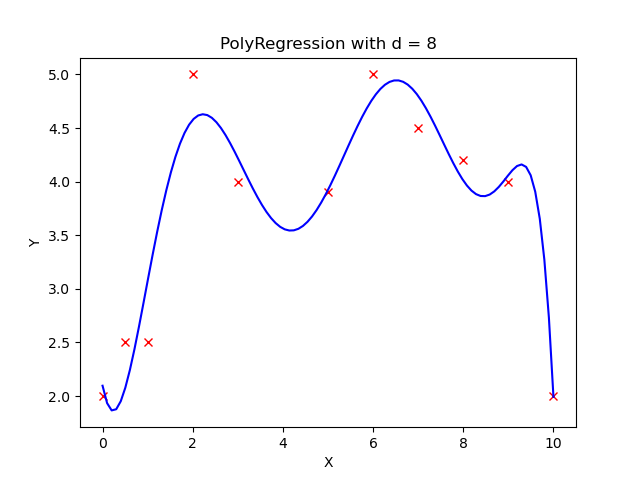
\includegraphics[width=\textwidth]{no_reg_plot.png}
                    \caption{Plot with no regularization}
                    \label{fig:no_reg_plot}
                \end{subfigure}
                \hfill
                \begin{subfigure}[b]{0.45\textwidth}
                    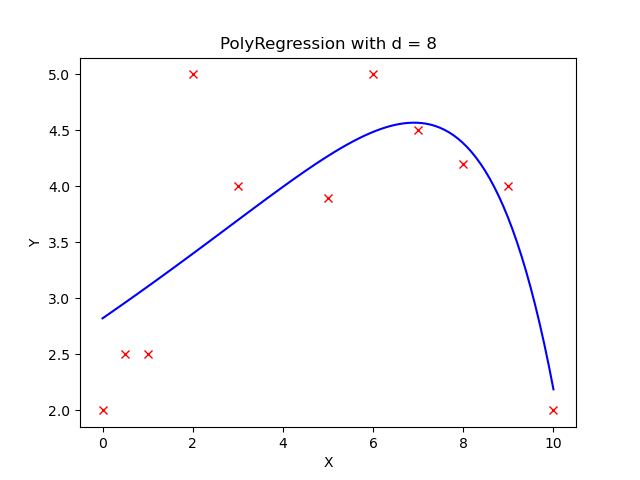
\includegraphics[width=\textwidth]{reg_1_plot.png}
                    \caption{Plot with regularization $\lambda = 1$}
                    \label{fig:reg_1_plot}
                \end{subfigure}
                \caption{Comparison of plots}
            \end{figure}
            As you can see, when you increase the regularization, the model tends to look less complex / overfit. For example, on the left the model is trying extremely hard to overfit the 12 data points, but on the right it looks like it took a more averaging approach. Realistically, small changes in the input should not lead to large changes in the output, like in figure (a).
        \end{enumerate}

        \item Here are the learning curves:
        \begin{figure}[H]
            \centering
            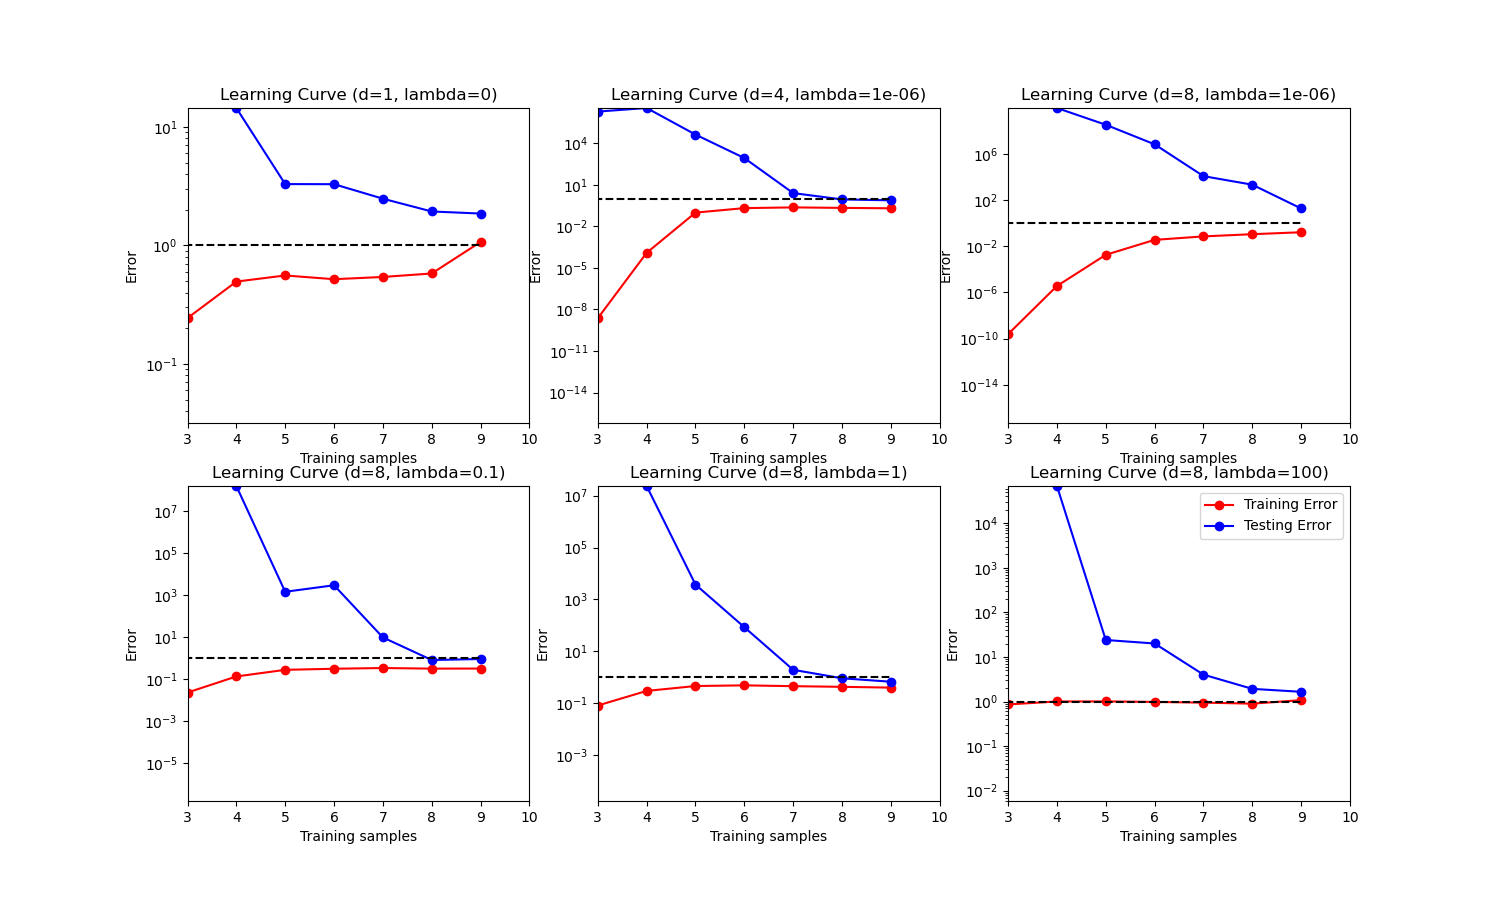
\includegraphics[width=\textwidth]{learning_curve.png}
            \caption{Learning curve for the model}
            \label{fig:learning_curve}
        \end{figure}

        \item \begin{enumerate}
            \item By definition, $\mg{W}_F^2 = \sum_{i,j} w_{ij}^2$. We see then that $\pdv{w_{ij}} \mg{W}_F^2 = 2w_{ij}$, which shows that $\grad_W \mg{W}_F^2 = 2W$. Per the hint, we know that 
            \begin{align*}
                \sum_{i=1}^n \mg{W^Tx_i - y_i}_2^2 = \sum_{j=1}^k \mg{Xw_j-Ye_j}_2^2
            \end{align*}
            We see now that, if $f(W) = \sum_{i=1}^n \mg{W^Tx_i-y_i}_2^2$,
            \begin{align*}
                \grad_{w_j} \sum_{j=1}^{k}\mg{Xw_j-Ye_j}_2^2 &= \grad_{w_j} \mg{Xw_j-Ye_j}_2^2 \\
                &= \grad_{w_j} (Xw_j-Ye_j)^T(Xw_j-Ye_j) \\
                &= \grad_{w_j} w_j^TX^TXw_j - 2e_j^TY^TXw_j \\
                &= 2X^TXw_j - 2X^TYe_j
            \end{align*}
            That is, the $j$th column of $\grad_W f(W)$ is $2X^TXw_j - 2X^TYe_j$, so $\grad_W f(W) = 2X^TXW - 2X^TY$. Thus the gradient of $g(W) = F(W) + \lambda \mg{W}_F^2$ is just $2X^TXW - 2X^TY + 2\lambda W$. Setting this to zero shows that $(X^TX+\lambda I)W = X^TY$, which shows that $\widehat{W} = (X^TX+\lambda I)^{-1}X^TY$.

            \item The training error I got was $14.805\%$ and the test error was $14.66\%$.
            \item Here is the plot of 10 samples:
            \begin{figure}[H]
                \centering
                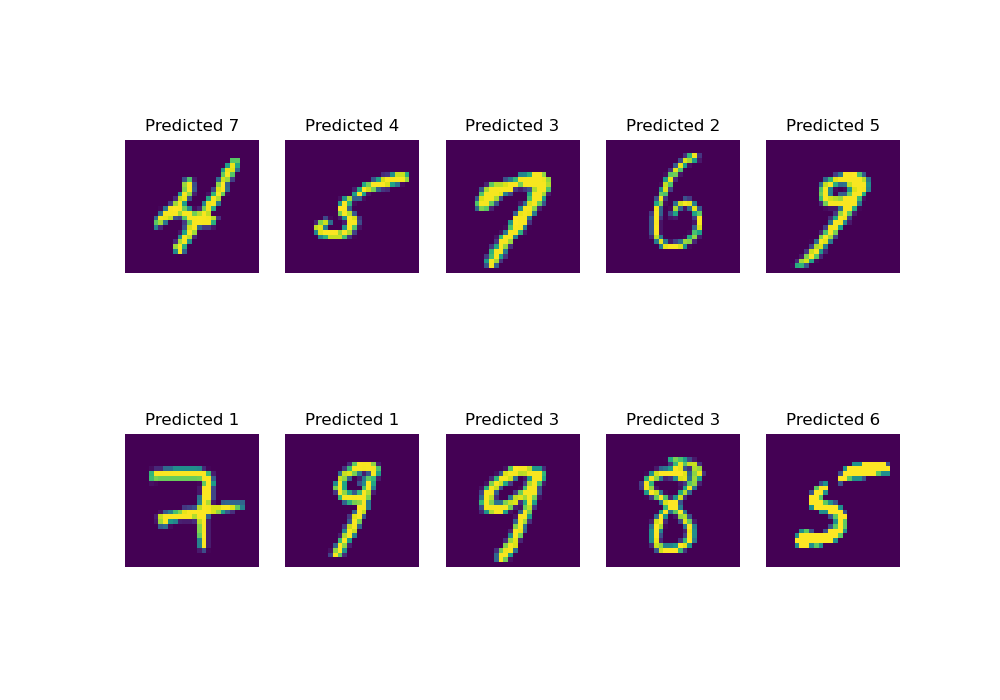
\includegraphics[width=\textwidth]{10_wrong_numbers.png}
                \caption{10 samples of wrong numbers}
                \label{fig:10_wrong_numbers}
            \end{figure}
            The big pattern I notice is that most of the numbers that it wrongly predicted seemed to be tilted left or right or disconnected. After looking at the numbers the model got right, most of these features did not show up in those samples.
        \end{enumerate}

        \item This assignment took me around 10 hours.
    \end{enumerate}
\end{document}
